\documentclass[10pt,a4paper]{article}
    \usepackage[a4paper, total={6.5in, 8in}, textheight = 700pt]{geometry}
    \usepackage[utf8]{inputenc}
    \usepackage{fancyhdr}
    \usepackage{listings}
    % \usepackage{minted}
    \usepackage{amsmath}
    \usepackage{amsfonts}
    \usepackage{amssymb}
    \usepackage{graphicx}
    \usepackage{wrapfig}
    \usepackage{caption}
    \usepackage{subcaption}
    \usepackage{float}
    \usepackage[space]{grffile}
    \usepackage{hyperref}
    \usepackage{multirow}
    \usepackage{booktabs}
    \usepackage{amsmath}
    \usepackage{multicol}
    \usepackage{enumitem}
    \usepackage{pageslts}
    \usepackage{setspace}
    \usepackage{color}
    \usepackage{xcolor}
    \usepackage{array}
    \usepackage{enumitem}
    \usepackage{libertine}
    \usepackage{lscape}
    \usepackage{pdfpages}
    \usepackage{pdflscape}
    \usepackage{tcolorbox}
    %% \usepackage[switch, modulo]{lineno}

    %%%%%%%%%%%%% PAGE LAYOUT %%%%%%%%%%%%%
    %\setstretch{1.25}
    %\textwidth=16.5cm
    %\textheight=24cm
    %\voffset=-60pt
    %\hoffset=-60pt
    \setlength{\parindent}{0cm} %No indentation in new paragraph
    \newcommand{\HRule}{\rule{\linewidth}{0.5mm}}
    \pagestyle{fancy}
    \fancyhf{} 
    %%%%%%%%%%%%% PAGE LAYOUT %%%%%%%%%%%%%
    
    
    %%%%%%%%%%%%% HEADER / FOOTER %%%%%%%%%%%%%
    \lhead{Gruppe 13} % Skriv gruppe nummer/navn her
    \chead{CDIO-Final} % Titel på projektet
    \rhead{Juni 2018} % Afleverings måned
    %%%%%%%%%%%%% HEADER / FOOTER %%%%%%%%%%%%%
    
    %%%%%%%%%%%%% BEGIN DOCUMENT %%%%%%%%%%%%%
    \begin{document}
    \pagenumbering{arabic}
    \thispagestyle{plain}
    %%%%%%%%%%%%% BEGIN DOCUMENT %%%%%%%%%%%%%
    
    %%%%%%%%%%%%% FRONT PAGE %%%%%%%%%%%%%
    \begin{titlepage}
\begin{center}


\includegraphics{Pictures/frontpage/dtu-logo.png}~\\[0.5cm]
\textsc{\Large Sens MOTION } \\% Kursus navn1

% Title
\HRule 
{ \huge \bfseries CDIO Final \\[0.1cm] } % Titel på projekt

\HRule \\[0.8cm]
\textsc{Gruppe 6}
%%% NEED FIX %%%
\begin{multicols}{5}
\begin{figure}[H]
        \centering
        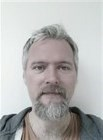
\includegraphics[scale=0.8]{Pictures/frontpage/kim.png}\\
        \textsc{Kim Sandberg Bossen}
        
        \textsc{s163290}\\
        \hfill \break
        \hfill \break
    \end{figure}
\columnbreak
    \begin{figure}[H]
        \centering
        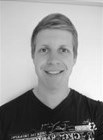
\includegraphics[scale=0.6]{Pictures/frontpage/Thyge.png}\\
        \textsc{Thyge S. Steffensen}
        
        \textsc{s175176}\\
        \hfill \break
        \hfill \break
    \end{figure}
\columnbreak
    \begin{figure}[H]
        \centering
        
\includegraphics[scale=0.8]{Pictures/frontpage/mathias.png}\\
        \textsc{Mathias M. Thejsen}
        
        \textsc{s175192}\\
        \hfill \break
        \hfill \break
    \end{figure}
\columnbreak
    \begin{figure}[H]
        \centering
        
\includegraphics[scale=0.8]{Pictures/frontpage/jeppe.png}\\
        \textsc{Jeppe Trip \\Kofoed}
        
        \textsc{s175197}\\
        \hfill \break
        \hfill \break
    \end{figure}
\columnbreak
    \begin{figure}[H]
        \centering
        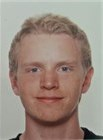
\includegraphics[scale=0.8]{Pictures/frontpage/christian.png}\\
        \textsc{Christian Stahl Andersen}
        
        \textsc{s164150}\\
        \hfill \break
        \hfill \break
    \end{figure}
\end{multicols}
\flushleft
\centering \today % Dags dato
\vfill
\flushleft
\centering \textit{\href{http://207.154.253.254:8080/13\_CDIO\_FINAL/}{http://207.154.253.254:8080/13\_CDIO\_FINAL/}}
\vfill
\end{center}

\end{titlepage}

    %%%%%%%%%%%%% FRONT PAGE %%%%%%%%%%%%%
    
    
    %%%%%%%%%%%%% TABLE OF CONTENT %%%%%%%%%%%%%
    \newpage
    \tableofcontents
    \cleardoublepage
    \cfoot{Page \thepage\ of \lastpageref{LastPage}}
    %%%%%%%%%%%%% TABLE OF CONTENT %%%%%%%%%%%%%
    
    %%%%%%%%%%%%% AFTER TABLE OF CONTENT %%%%%%%%%%%%%
    \setcounter{page}{1}
    \def\emptyline{\vspace{12pt}}
     
    
    \end{document}
\begin{document}
\begin{itemize}

\item A brief text description of the deliverable including objective of the iteration
\item Core user stories
\item Brief explanatory text of the user goals/tasks implemented and the flow/navigation supported by e.g. flow/navigation diagram from Adobe XD
\item A link to the interactive prototype and possibly the Adobe XD or Justinmind mobile app, allowing the prototype to be downloaded on a mobile. Permissions and instructions in order to use prototype should be provided.
\item Clarifying questions for the project provider relating to any uncertainties, if necessary.
\item If time allows, a higher fidelity prototype can also be delivered to discuss initial design ideas and concepts.
\end{itemize}

\section{User stories}
\begin{itemize}
\item Som en patient, vil jeg gerne kunne se en måling over mit nuværende aktivitetsniveau, så jeg ved hvordan jeg ligger i forhold til mine mål.
\item Som en patient, vil jeg gerne kunne se en oversigt over tidligere aktiviteter for at se udviklingen i aktivitetsniveau.
\item Som patient vil jeg gerne motiveres til at bevæge mig så jeg styrker min evne til at skabe gode vaner omkring bevægelse. 
\item Som patient når jeg ser min aktivitet så jeg nemt kan overskue og forstå hvordan det går.
\item Som patient vil jeg gerne blive påmindet om mit aktivitetsniveau, for at blive motiveret til at bevæge mig mere.
\item Som patient vil jeg gerne kunne logge ind for at tilgå personlig bevægelsesdata.
\item Som patient vil jeg gerne kunne vælge mellem grafer eller det interaktive spil for at se det jeg finder mest relevant.
\item Som patient vil jeg gerne kunne skrive mit brugerid for at logge ind.
\end{itemize}



\end{document}
